% Figure 5: literature evidence and numerical-subspace deletion.
\begin{figure*}[t]
\centering
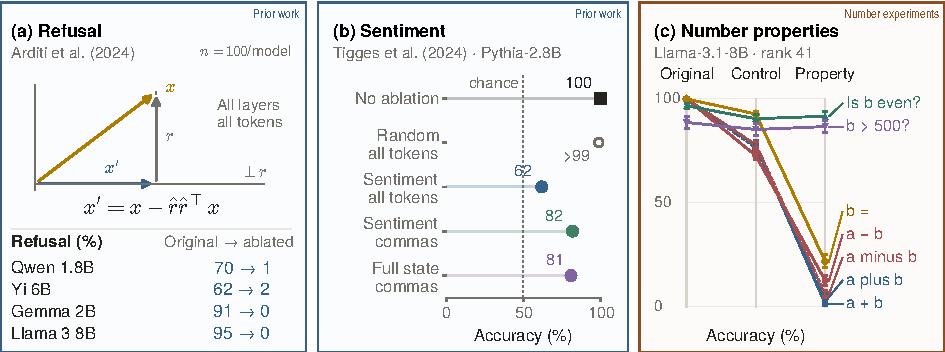
\includegraphics[width=\textwidth]{../figures/fig_causal_use_space_optimized.pdf}
\caption{Direction ablation and subspace deletion test causal necessity through changes in behavior.
(a) Removing an activation's component along the refusal direction suppresses refusal on harmful instructions in four models \citep{arditi2024refusal}.
(b) Ablating a sentiment direction lowers accuracy on originally correct SST examples containing commas \citep{tigges2023linear}.
(c) Deleting the subspace fitted to number properties impairs arithmetic and copying more than parity and comparison.
\emph{Property} and \emph{Control} delete rank-41 spans fitted on addition formulas with true or shuffled property labels.
The contrast with \emph{Control} supports a behavioral role for the property subspace.
Whiskers in (c) give 95\% source-value-cluster bootstrap intervals, conditional on ten fitted bases.}
\label{fig:causal-use}
\end{figure*}
